\documentclass[11pt]{handout}
\usepackage{moreverb}
\usepackage{tabularx}
\usepackage{epsf}
\usepackage{epic}
\usepackage{eepic}
\usepackage{epsfig}
\usepackage{epsf}
\usepackage{fancyheadings}
\usepackage{fancybox}

\renewcommand{\coursetitle}{ECE 320}
\renewcommand{\handouttitle}{Carrier Recovery}
\renewcommand{\handoutauthor}{Michael Kramer}
\renewcommand{\semestertitle}{Spring 2000}

\newcommand{\blt}{\mbox{$\bullet$ }}

\newcommand{\bea}{\begin{eqnarray}}
\newcommand{\eea}{\end{eqnarray}}

\setlength{\parindent}{5mm}
\begin{document}

\setlength{\baselineskip}{0.5cm}
\setlength{\parskip}{0.5cm}

\makeboxtitle
\vspace{0.3cm}

\section{Introduction:}

This handout is designed to provide you with a brief
description on the carrier recovery sub-system of a digital receiver 
and addresses some of the details associated with its 
implementation/simulation in \matlab and on the DSP.
The sub-system covered is specifically tailored to a
non-modulated carrier.  In the final PLL implementation used for
your digital receiver you will have to make modifications
to the specific details mentioned.


%
% 
% Module: carrier_recovery_theory_tutorial
%
% Author: Michael Kramer
%
%

The phase locked loop is a critical component in coherent communications
receivers that is responsible for locking onto the carrier of a received 
modulated signal.  
Ideally the transmitted carrier frequency is known and we need
to know its phase for accurate demodulation.  However, due
to imperfections at the transmitter, the actual carrier frequency
may be slightly different than the expected frequency.  For example, in the 
QPSK transmitter of Lab 5 if the digital carrier frequency is $\frac{\pi}{2}$
and the D/A is operating at 44.1 kHz, then the expected analog carrier 
frequency is $f_c = \frac{\frac{\pi}{2}}{2 \pi} * 44.1 \: kHz \: = 11.025 kHz$.
If there is a slight change to the D/A sample rate 
(say $F_s = 44.05 kHz$) then there will be a corresponding 
change in the actual analog carrier frequency ($f_c = 11.0125 \: kHz$).

This difference between the expected and actual carrier frequencies
can be modeled as a time-varying phase.  
Provided that the frequency mismatch is small relative to the
carrier frequency, the feed-back control of an appropriately
calibrated PLL can track this time-varying phase, thereby locking
onto the correct frequency as well as phase.

\begin{figure}[ht]
   \begin{center}
      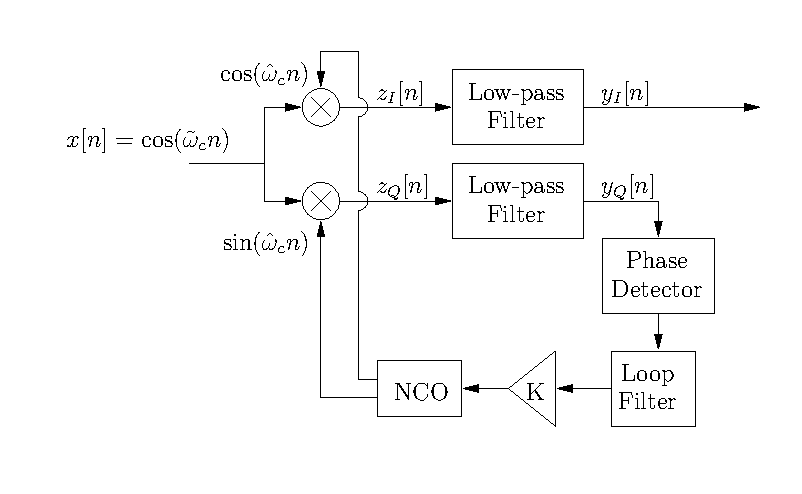
\epsfig{file=pll.eps,width=10cm}
      \caption{PLL block diagram.}
      \label{fig: PLL}
   \end{center}
\end{figure}

\paragraph{Numerically Controlled Oscillator:}

In a complete coherent receiver implementation, carrier
recovery is required since the receiver typically does not know
the exact phase and frequency of the transmitted carrier.
In an analog system this recovery is often implemented with
a voltage-controlled oscillator (VCO) that allows for precise
adjustment of the carrier frequency based on the output of
a phase detecting circuit.

In our digital application, this adjustment is performed
with a numerically controlled oscillator (NCO) (see Figure
\ref{fig: PLL}).  A simple
scheme for implementing an NCO is based on the following
re-expression of the carrier sinusoid
\bea
\sin(\lambda_c n + \theta_c) & = & \sin ( \theta(n) ) \nonumber 
\eea
where $\theta(n) = \lambda_c n + \theta_c$ ($\lambda_c$ and $\theta_c$
represent the carrier frequency and phase respectively).
This time-varying phase term can be expressed as $\theta(n) = 
\left( \sum_{m=0}^{n} \lambda_c \right) + \theta_c$ and then recursively as
\bea
\theta(n) & = & \theta(n-1) + \lambda_c
\eea
The NCO can keep track of the phase, $\theta(n)$, and force a phase offset
in the demodulating carrier by incorporating an extra term in this
recursive update
\bea
\theta(n) & = & \theta(n-1) + \lambda_c + \delta_{pd}(n)
\label{eq: phase_update}
\eea
where $\delta_{pd}(n)$ is the amount of desired phase offset
at time $n$. (What would $\delta_{pd}(n)$ look like to generate
a frequency offset?)

\paragraph{Phase Detector:}

The goal of the PLL is to maintain a demodulating sine
and cosine that match the incoming carrier frequency.
Suppose $\lambda_c$ is the believed digital
carrier frequency.  We can then represent the actual 
received carrier frequency as the expected carrier frequency
with some offset, $\tilde{\lambda}_c n = \lambda_c n + \tilde{\theta}(n)$.
The NCO generates the demodulating sine and cosine with 
the expected digital frequency $\lambda_c$ and offsets this
frequency with the output of the loop filter.  The NCO
frequency can then be modeled as $\hat{\lambda}_c n = \lambda_c n
+ \hat{\theta}(n)$.  
Using the appropriate trigonometric identities\footnote{
$\cos(A) \cos(B) = \frac{1}{2} \left[ \cos (A-B) + \cos(A+B) \right]$
and 
$\cos(A) \sin(B) = \frac{1}{2} \left[ \sin (B-A) + \sin(A+B) \right]$
}, the in-phase
and quadrature signals can be expressed as
\bea
z_I(n) & = & \frac{1}{2} \left[ \cos (\tilde{\theta}(n) - \hat{\theta}(n) )
+ \cos ( 2 \lambda_c + \tilde{\theta}(n) + \hat{\theta}(n) ) \right]
\nonumber\\
z_Q(n) & = & \frac{1}{2} \left[ \sin (\hat{\theta}(n) - \tilde{\theta}(n) )
+ \sin ( 2 \lambda_c + \tilde{\theta}(n) + \hat{\theta}(n) ) \right]
\eea
After applying a low-pass filter to remove the double frequency
terms we have
\bea
y_I(n) & = & \frac{1}{2}  \cos (\tilde{\theta}(n) - \hat{\theta}(n) )
\nonumber\\
y_Q(n) & = & \frac{1}{2}  \sin (\hat{\theta}(n) - \tilde{\theta}(n))
\eea

Note that the quadrature signal, $z_Q(n)$, is zero
when the received carrier and internally generated 
waves are exactly matched in frequency and phase.  When the phases 
are only slightly mismatched we can use the relation
\bea
\sin(\theta) \approx \theta & &\mbox{ for small } \theta \nonumber
\eea
and let the current value of the quadrature channel approximate the
phase difference: $z_Q(n) \approx (\hat{\theta}(n) - \tilde{\theta}(n))$.
With the exception of the sign error, this difference is essentially how 
much we need to offset our NCO frequency by 
(if $(\hat{\theta}(n) - \tilde{\theta}(n)) >0$
then $\hat{\theta}(n)$ is too large and we want to decrease our NCO
phase)
To make sure that the sign of the phase estimate is right,
in this example the phase detector is simply minus-one times
the value of the quadrature signal.  
In a more advanced receiver, information from both the in-phase
and quadrature branches is used to generate an estimate of
the phase error.  (What should the relationship between the I and Q
branches be for a digital QPSK signal?)

\paragraph{Loop Filter:}

The estimated phase mismatch estimate is fed to the NCO via a loop-filter,
often a simple low-pass filter. For this exercise you can use a 1-tap 
IIR filter,
\bea
y(n) & = & \beta x(n) + \alpha y(n-1)
\eea
To ensure that the DC term of the filter is at unity gain we select
$\beta = 1 - \alpha$.

It is suggested that you start by choosing $\alpha = 0.6$ and $K = 0.15$ 
for the loop-gain.  Once you have a working system, investigate
the effects of modifying these values.


\section{Matlab Simulation:}


%
%
% Module: carrier_recovery_matlab_exercise
%
% Author: Michael Kramer
%
%

Simulate the PLL system shown in Figure \ref{fig: PLL} using
\matlab.  As with the DLL simulation, you will have to simulate
the PLL on a sample by sample basis. 

Use equation (\ref{eq: phase_update}) to implement your NCO in 
\matlab. However to ensure that the phase term does not grow
to infinity you should use addition modulo $2 \pi$ in the phase update
relation.  This can be done by checking to see if $\theta(n) > 2 \pi$,
and if so, replace it with $\theta(n) = \theta(n) - 2 \pi$.

Figure \ref{fig: pll_output} illustrates how the proposed PLL will
behave when given a modulated BPSK waveform.  In this case
the transmitted carrier frequency was set to $\tilde{\lambda}_c =
\frac{\pi}{2} + \frac{\pi}{1024}$ to simulate a frequency offset.

\begin{figure}[ht]
   \begin{center}
      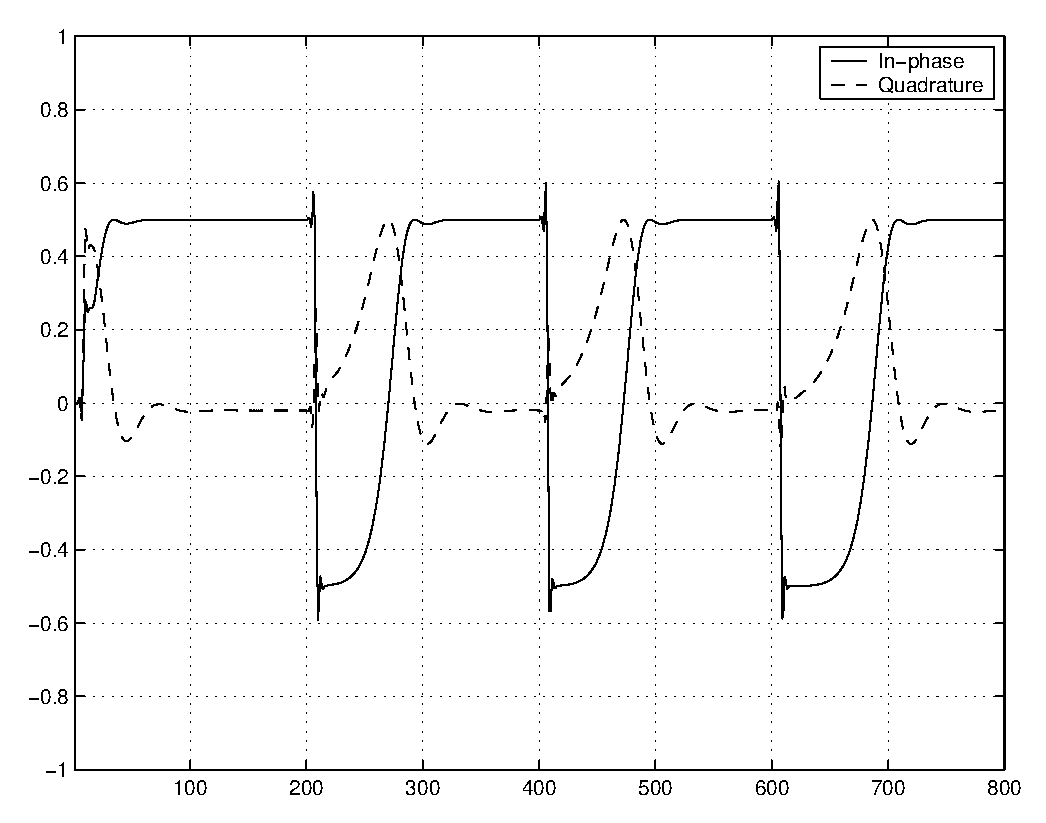
\epsfig{file=pll_output.eps,width=10cm}
      \caption{Output of PLL sub-system for BPSK modulated carrier.}
      \label{fig: pll_output}
   \end{center}
\end{figure}

Note that each time an amplitude transition occurs in the BPSK
waveform, this is equivalent to a phase shift of the carrier
by $\frac{\pi}{2}$.  Immediately after this phase change occurs
the PLL begins to adjust the phase to force the quadrature
component to zero (and the in-phase component to $\frac{1}{2}$).
Why would this phase detector not work in a real BPSK environment?


\section{DSP Implementation:}

As you begin to implement your PLL on the DSP it is highly
recommended that you implement and 
test your NCO block first before completing the rest
of the phase-locked loop.


%
%
% Module: carrier_recovery_processor_exercise
%
% Author: Michael Kramer
%
%

\paragraph{Sine Table Interpolation:}

Because
we must be able to finely adjust the oscillating (carrier) frequency,
some form of interpolation is required to generate our
demodulating sine and cosine using table look-up.
With the following sine table in memory: $\sin(\frac{2\pi}{N}k)$
for $k=0, ..., N-1$, we can generate a sine wave by incrementing
through the table.  If we skip through the table by $p$ samples
then we would generate a sine wave with a digital frequency of
$\lambda = \frac{2 \pi}{N} p$. 
In contrast to this method where the carrier
wave is generated by stepping through the sine
table by integral amounts, the demodulating sinusoids
in this exercise will be generated
using a mixed integer / fractional index.
This enables much more precise frequency adjustment of the demodulating
carrier. 


Typically one would use an address register and increment it by
an appropriate amount to generate the desired frequencies.  For
non-integral increments through the sine table a non-integral
``pointer'' must be used.  This pointer can interpreted as the phase
of equation (\ref{eq: phase_update}). To generate a sine sample indexed
by a non-integral pointer we can simply round the value
down to the nearest integer and then use it as a regular integer
pointer to our sine-table. 
Although this method of interpolation (also referred to
as a zero-order hold interpolator) is rather crude, for a
long enough sine table this approximation is good enough to 
finely adjust the NCO frequency for this application. 

To implement a non-integral pointer we can perform addition
in the accumulator with a modified decimal point.  For
example, with $N=256$ we need 8 bits to represent the
integer portion of our pointer.  If we interpret the 
lower 16 bits of the accumulator
to have a decimal point seven bits up
from the bottom, then there are still nine bits of space for 
an integer above this decimal point.
To step through the sine table we
can then add a 15-bit value to the low-part of the
accumulator, then mask off the top bit to ensure that
the value in the accumulator is between $0$ and $255.99999$
(this is similar to the modulo addition of $2 \pi$ discussed
in the \matlab Simulation section:  Why?)
To use only the integer portion of the ``pointer'' we
can shift the accumulator down by seven bits, then store
the low part into an address register, \verb+ARX+.  After adding the
start of the sine table to the \verb+ARX+ register we are now 
ready to look-up the approximating sample out of the sine table.
 
As an example, if we want the carrier frequency to be
$\lambda = \frac{\pi}{8}$, the integer step size 
would be $p=\frac{N}{16} = 8$.  When the decimal
place is interpreted as being 7 bits up from the 
bottom of the register, the corresponding value
to increment by would be $8 \times 2^7 = 1024$. 
(What would the output frequency be if this step size was
set to 1025?)


\section{Extensions}

As your final project will require some modification to the discussed
non-modulated carrier recovery, you will want to refer to the listed 
references, \cite{Proakis1, Blahut1},
and consider some of the following questions regarding such 
modifications:

\blt How does the addition of noise affect the described carrier recovery 
method?

\blt What should the phase-detector look like for a BPSK modulated carrier?

\vspace*{-.1in}
\hspace{.1in} (Hint: you now need to consider both the in-phase and 
quadrature channels.)

\blt How does $\alpha$ affect the bandwidth of the loop-filter?

\blt How does the loop-gain, $K$, and the bandwidth of the loop-filter
affect the PLL's ability to lock onto a carrier frequency mismatch?

\bibliographystyle{ieeetr}
\bibliography{../../ece320}


\end{document}
\bye
